\documentclass[1p]{elsarticle_modified}
%\bibliographystyle{elsarticle-num}

%\usepackage[colorlinks]{hyperref}
%\usepackage{abbrmath_seonhwa} %\Abb, \Ascr, \Acal ,\Abf, \Afrak
\usepackage{amsfonts}
\usepackage{amssymb}
\usepackage{amsmath}
\usepackage{amsthm}
\usepackage{scalefnt}
\usepackage{amsbsy}
\usepackage{kotex}
\usepackage{caption}
\usepackage{subfig}
\usepackage{color}
\usepackage{graphicx}
\usepackage{xcolor} %% white, black, red, green, blue, cyan, magenta, yellow
\usepackage{float}
\usepackage{setspace}
\usepackage{hyperref}

\usepackage{tikz}
\usetikzlibrary{arrows}

\usepackage{multirow}
\usepackage{array} % fixed length table
\usepackage{hhline}

%%%%%%%%%%%%%%%%%%%%%
\makeatletter
\renewcommand*\env@matrix[1][\arraystretch]{%
	\edef\arraystretch{#1}%
	\hskip -\arraycolsep
	\let\@ifnextchar\new@ifnextchar
	\array{*\c@MaxMatrixCols c}}
\makeatother %https://tex.stackexchange.com/questions/14071/how-can-i-increase-the-line-spacing-in-a-matrix
%%%%%%%%%%%%%%%

\usepackage[normalem]{ulem}

\newcommand{\msout}[1]{\ifmmode\text{\sout{\ensuremath{#1}}}\else\sout{#1}\fi}
%SOURCE: \msout is \stkout macro in https://tex.stackexchange.com/questions/20609/strikeout-in-math-mode

\newcommand{\cancel}[1]{
	\ifmmode
	{\color{red}\msout{#1}}
	\else
	{\color{red}\sout{#1}}
	\fi
}

\newcommand{\add}[1]{
	{\color{blue}\uwave{#1}}
}

\newcommand{\replace}[2]{
	\ifmmode
	{\color{red}\msout{#1}}{\color{blue}\uwave{#2}}
	\else
	{\color{red}\sout{#1}}{\color{blue}\uwave{#2}}
	\fi
}

\newcommand{\Sol}{\mathcal{S}} %segment
\newcommand{\D}{D} %diagram
\newcommand{\A}{\mathcal{A}} %arc


%%%%%%%%%%%%%%%%%%%%%%%%%%%%%5 test

\def\sl{\operatorname{\textup{SL}}(2,\Cbb)}
\def\psl{\operatorname{\textup{PSL}}(2,\Cbb)}
\def\quan{\mkern 1mu \triangleright \mkern 1mu}

\theoremstyle{definition}
\newtheorem{thm}{Theorem}[section]
\newtheorem{prop}[thm]{Proposition}
\newtheorem{lem}[thm]{Lemma}
\newtheorem{ques}[thm]{Question}
\newtheorem{cor}[thm]{Corollary}
\newtheorem{defn}[thm]{Definition}
\newtheorem{exam}[thm]{Example}
\newtheorem{rmk}[thm]{Remark}
\newtheorem{alg}[thm]{Algorithm}

\newcommand{\I}{\sqrt{-1}}
\begin{document}

%\begin{frontmatter}
%
%\title{Boundary parabolic representations of knots up to 8 crossings}
%
%%% Group authors per affiliation:
%\author{Yunhi Cho} 
%\address{Department of Mathematics, University of Seoul, Seoul, Korea}
%\ead{yhcho@uos.ac.kr}
%
%
%\author{Seonhwa Kim} %\fnref{s_kim}}
%\address{Center for Geometry and Physics, Institute for Basic Science, Pohang, 37673, Korea}
%\ead{ryeona17@ibs.re.kr}
%
%\author{Hyuk Kim}
%\address{Department of Mathematical Sciences, Seoul National University, Seoul 08826, Korea}
%\ead{hyukkim@snu.ac.kr}
%
%\author{Seokbeom Yoon}
%\address{Department of Mathematical Sciences, Seoul National University, Seoul, 08826,  Korea}
%\ead{sbyoon15@snu.ac.kr}
%
%\begin{abstract}
%We find all boundary parabolic representation of knots up to 8 crossings.
%
%\end{abstract}
%\begin{keyword}
%    \MSC[2010] 57M25 
%\end{keyword}
%
%\end{frontmatter}

%\linenumbers
%\tableofcontents
%
\newcommand\colored[1]{\textcolor{white}{\rule[-0.35ex]{0.8em}{1.4ex}}\kern-0.8em\color{red} #1}%
%\newcommand\colored[1]{\textcolor{white}{ #1}\kern-2.17ex	\textcolor{white}{ #1}\kern-1.81ex	\textcolor{white}{ #1}\kern-2.15ex\color{red}#1	}

{\Large $\underline{11n_{116}~(K11n_{116})}$}

\setlength{\tabcolsep}{10pt}
\renewcommand{\arraystretch}{1.6}
\vspace{1cm}\begin{tabular}{m{100pt}>{\centering\arraybackslash}m{274pt}}
\multirow{5}{120pt}{
	\centering
	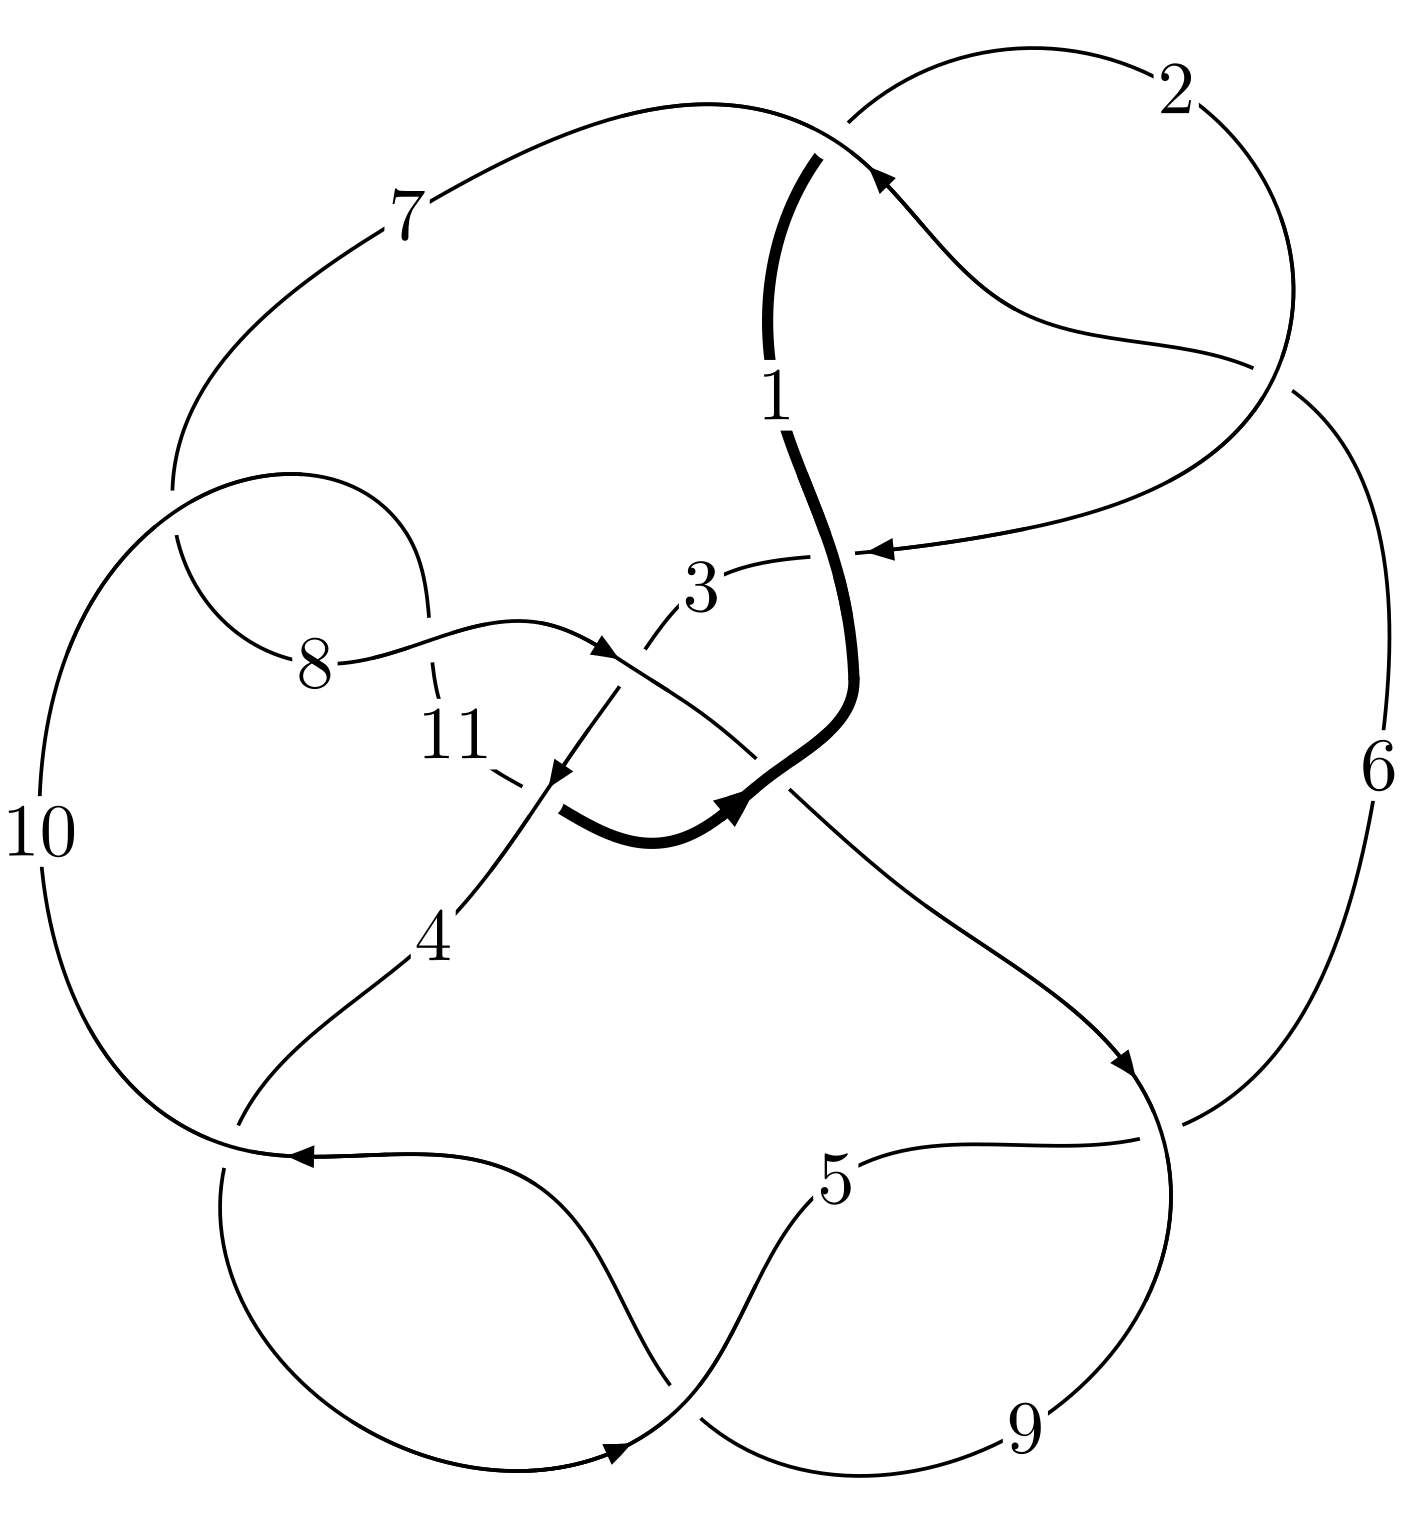
\includegraphics[width=112pt]{../../../GIT/diagram.site/Diagrams/png/732_11n_116.png}\\
\ \ \ A knot diagram\footnotemark}&
\allowdisplaybreaks
\textbf{Linearized knot diagam} \\
\cline{2-2}
 &
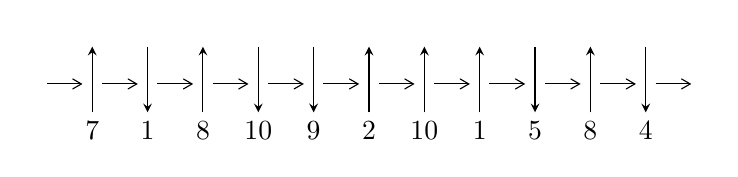
\begin{tikzpicture}[x=20pt, y=17pt]
	% nodes
	\node (C0) at (0, 0) {};
	\node (C1) at (1, 0) {};
	\node (C1U) at (1, +1) {};
	\node (C1D) at (1, -1) {7};

	\node (C2) at (2, 0) {};
	\node (C2U) at (2, +1) {};
	\node (C2D) at (2, -1) {1};

	\node (C3) at (3, 0) {};
	\node (C3U) at (3, +1) {};
	\node (C3D) at (3, -1) {8};

	\node (C4) at (4, 0) {};
	\node (C4U) at (4, +1) {};
	\node (C4D) at (4, -1) {10};

	\node (C5) at (5, 0) {};
	\node (C5U) at (5, +1) {};
	\node (C5D) at (5, -1) {9};

	\node (C6) at (6, 0) {};
	\node (C6U) at (6, +1) {};
	\node (C6D) at (6, -1) {2};

	\node (C7) at (7, 0) {};
	\node (C7U) at (7, +1) {};
	\node (C7D) at (7, -1) {10};

	\node (C8) at (8, 0) {};
	\node (C8U) at (8, +1) {};
	\node (C8D) at (8, -1) {1};

	\node (C9) at (9, 0) {};
	\node (C9U) at (9, +1) {};
	\node (C9D) at (9, -1) {5};

	\node (C10) at (10, 0) {};
	\node (C10U) at (10, +1) {};
	\node (C10D) at (10, -1) {8};

	\node (C11) at (11, 0) {};
	\node (C11U) at (11, +1) {};
	\node (C11D) at (11, -1) {4};
	\node (C12) at (12, 0) {};

	% arrows
	\draw[->,>={angle 60}]
	(C0) edge (C1) (C1) edge (C2) (C2) edge (C3) (C3) edge (C4) (C4) edge (C5) (C5) edge (C6) (C6) edge (C7) (C7) edge (C8) (C8) edge (C9) (C9) edge (C10) (C10) edge (C11) (C11) edge (C12) ;	\draw[->,>=stealth]
	(C1D) edge (C1U) (C2U) edge (C2D) (C3D) edge (C3U) (C4U) edge (C4D) (C5U) edge (C5D) (C6D) edge (C6U) (C7D) edge (C7U) (C8D) edge (C8U) (C9U) edge (C9D) (C10D) edge (C10U) (C11U) edge (C11D) ;
	\end{tikzpicture} \\
\hhline{~~} \\& 
\textbf{Solving Sequence} \\ \cline{2-2} 
 &
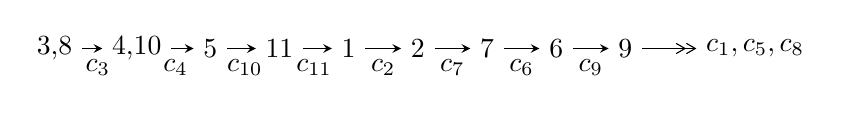
\begin{tikzpicture}[x=25pt, y=7pt]
	% node
	\node (A0) at (-1/8, 0) {3,8};
	\node (A1) at (17/16, 0) {4,10};
	\node (A2) at (17/8, 0) {5};
	\node (A3) at (25/8, 0) {11};
	\node (A4) at (33/8, 0) {1};
	\node (A5) at (41/8, 0) {2};
	\node (A6) at (49/8, 0) {7};
	\node (A7) at (57/8, 0) {6};
	\node (A8) at (65/8, 0) {9};
	\node (C1) at (1/2, -1) {$c_{3}$};
	\node (C2) at (13/8, -1) {$c_{4}$};
	\node (C3) at (21/8, -1) {$c_{10}$};
	\node (C4) at (29/8, -1) {$c_{11}$};
	\node (C5) at (37/8, -1) {$c_{2}$};
	\node (C6) at (45/8, -1) {$c_{7}$};
	\node (C7) at (53/8, -1) {$c_{6}$};
	\node (C8) at (61/8, -1) {$c_{9}$};
	\node (A9) at (10, 0) {$c_{1},c_{5},c_{8}$};

	% edge
	\draw[->,>=stealth]	
	(A0) edge (A1) (A1) edge (A2) (A2) edge (A3) (A3) edge (A4) (A4) edge (A5) (A5) edge (A6) (A6) edge (A7) (A7) edge (A8) ;
	\draw[->>,>={angle 60}]	
	(A8) edge (A9);
\end{tikzpicture} \\ 

\end{tabular} \\

\footnotetext{
The image of knot diagram is generated by the software ``\textbf{Draw programme}" developed by Andrew Bartholomew(\url{http://www.layer8.co.uk/maths/draw/index.htm\#Running-draw}), where we modified some parts for our purpose(\url{https://github.com/CATsTAILs/LinksPainter}).
}\phantom \\ \newline 
\centering \textbf{Ideals for irreducible components\footnotemark of $X_{\text{par}}$} 
 
\begin{align*}
I^u_{1}&=\langle 
8 u^7+2 u^6+43 u^5-42 u^4+38 u^3-164 u^2+17 b+20 u-27,\\
\phantom{I^u_{1}}&\phantom{= \langle  }28 u^7+58 u^6+244 u^5+278 u^4+490 u^3+191 u^2+17 a+53 u+33,\\
\phantom{I^u_{1}}&\phantom{= \langle  }u^8+2 u^7+9 u^6+10 u^5+20 u^4+8 u^3+7 u^2+u+1\rangle \\
I^u_{2}&=\langle 
56 u^7-6 u^6+421 u^5+108 u^4+1168 u^3+208 u^2+397 b+934 u+377,\\
\phantom{I^u_{2}}&\phantom{= \langle  }-418 u^7+300 u^6-2788 u^5+158 u^4-4408 u^3-475 u^2+1191 a-251 u-985,\\
\phantom{I^u_{2}}&\phantom{= \langle  }u^8+7 u^6+4 u^5+16 u^4+10 u^3+11 u^2+7 u+3\rangle \\
\\
\end{align*}
\raggedright * 2 irreducible components of $\dim_{\mathbb{C}}=0$, with total 16 representations.\\
\footnotetext{All coefficients of polynomials are rational numbers. But the coefficients are sometimes approximated in decimal forms when there is not enough margin.}
\newpage
\renewcommand{\arraystretch}{1}
\centering \section*{I. $I^u_{1}= \langle 8 u^7+2 u^6+\cdots+17 b-27,\;28 u^7+58 u^6+\cdots+17 a+33,\;u^8+2 u^7+\cdots+u+1 \rangle$}
\flushleft \textbf{(i) Arc colorings}\\
\begin{tabular}{m{7pt} m{180pt} m{7pt} m{180pt} }
\flushright $a_{3}=$&$\begin{pmatrix}1\\0\end{pmatrix}$ \\
\flushright $a_{8}=$&$\begin{pmatrix}0\\u\end{pmatrix}$ \\
\flushright $a_{4}=$&$\begin{pmatrix}1\\- u^2\end{pmatrix}$ \\
\flushright $a_{10}=$&$\begin{pmatrix}-1.64706 u^{7}-3.41176 u^{6}+\cdots-3.11765 u-1.94118\\-0.470588 u^{7}-0.117647 u^{6}+\cdots-1.17647 u+1.58824\end{pmatrix}$ \\
\flushright $a_{5}=$&$\begin{pmatrix}1.35294 u^{7}+0.588235 u^{6}+\cdots+6.88235 u-2.94118\\-2.70588 u^{7}-5.17647 u^{6}+\cdots-6.76471 u-3.11765\end{pmatrix}$ \\
\flushright $a_{11}=$&$\begin{pmatrix}-1.64706 u^{7}-3.41176 u^{6}+\cdots-3.11765 u-1.94118\\-1.17647 u^{7}-1.29412 u^{6}+\cdots-2.94118 u+1.47059\end{pmatrix}$ \\
\flushright $a_{1}=$&$\begin{pmatrix}-1.17647 u^{7}-3.29412 u^{6}+\cdots-1.94118 u-3.52941\\-1.11765 u^{7}-1.52941 u^{6}+\cdots-3.29412 u+0.647059\end{pmatrix}$ \\
\flushright $a_{2}=$&$\begin{pmatrix}-7.58824 u^{7}-14.6471 u^{6}+\cdots-17.4706 u-8.76471\\0.176471 u^{7}+2.29412 u^{6}+\cdots-5.05882 u+8.52941\end{pmatrix}$ \\
\flushright $a_{7}=$&$\begin{pmatrix}-1.64706 u^{7}-1.41176 u^{6}+\cdots-7.11765 u+3.05882\\2.41176 u^{7}+4.35294 u^{6}+\cdots+6.52941 u+3.23529\end{pmatrix}$ \\
\flushright $a_{6}=$&$\begin{pmatrix}-3.64706 u^{7}-12.4118 u^{6}+\cdots-1.11765 u-20.9412\\-6.70588 u^{7}-9.17647 u^{6}+\cdots-21.7647 u+2.88235\end{pmatrix}$ \\
\flushright $a_{9}=$&$\begin{pmatrix}6.52941 u^{7}+11.8824 u^{6}+\cdots+15.8235 u+6.58824\\-0.529412 u^{7}-2.88235 u^{6}+\cdots+3.17647 u-7.58824\end{pmatrix}$\\ \flushright $a_{9}=$&$\begin{pmatrix}6.52941 u^{7}+11.8824 u^{6}+\cdots+15.8235 u+6.58824\\-0.529412 u^{7}-2.88235 u^{6}+\cdots+3.17647 u-7.58824\end{pmatrix}$\\&\end{tabular}
\flushleft \textbf{(ii) Obstruction class $= -1$}\\~\\
\flushleft \textbf{(iii) Cusp Shapes $= -\frac{19}{17} u^7-\frac{60}{17} u^6-\frac{219}{17} u^5-\frac{389}{17} u^4-\frac{613}{17} u^3-\frac{571}{17} u^2-\frac{260}{17} u-\frac{57}{17}$}\\~\\
\newpage\renewcommand{\arraystretch}{1}
\flushleft \textbf{(iv) u-Polynomials at the component}\newline \\
\begin{tabular}{m{50pt}|m{274pt}}
Crossings & \hspace{64pt}u-Polynomials at each crossing \\
\hline $$\begin{aligned}c_{1},c_{6}\end{aligned}$$&$\begin{aligned}
&u^8+3 u^7+12 u^6+15 u^5+32 u^4+9 u^3+27 u^2-21 u+11
\end{aligned}$\\
\hline $$\begin{aligned}c_{2}\end{aligned}$$&$\begin{aligned}
&u^8+15 u^7+\cdots+153 u+121
\end{aligned}$\\
\hline $$\begin{aligned}c_{3}\end{aligned}$$&$\begin{aligned}
&u^8+2 u^7+9 u^6+10 u^5+20 u^4+8 u^3+7 u^2+u+1
\end{aligned}$\\
\hline $$\begin{aligned}c_{4},c_{5},c_{9}\end{aligned}$$&$\begin{aligned}
&u^8+8 u^6-4 u^5+36 u^4-29 u^3+41 u^2+17 u+19
\end{aligned}$\\
\hline $$\begin{aligned}c_{7},c_{10}\end{aligned}$$&$\begin{aligned}
&u^8+2 u^7+8 u^6+3 u^5+38 u^4-38 u^3+58 u^2-12 u+7
\end{aligned}$\\
\hline $$\begin{aligned}c_{8}\end{aligned}$$&$\begin{aligned}
&u^8-2 u^7+10 u^6+6 u^5+168 u^4+139 u^3+116 u^2-60 u+47
\end{aligned}$\\
\hline $$\begin{aligned}c_{11}\end{aligned}$$&$\begin{aligned}
&u^8-4 u^7+13 u^6-28 u^5+90 u^4+60 u^3+85 u^2+23 u+11
\end{aligned}$\\
\hline
\end{tabular}\\~\\
\newpage\renewcommand{\arraystretch}{1}
\flushleft \textbf{(v) Riley Polynomials at the component}\newline \\
\begin{tabular}{m{50pt}|m{274pt}}
Crossings & \hspace{64pt}Riley Polynomials at each crossing \\
\hline $$\begin{aligned}c_{1},c_{6}\end{aligned}$$&$\begin{aligned}
&y^8+15 y^7+\cdots+153 y+121
\end{aligned}$\\
\hline $$\begin{aligned}c_{2}\end{aligned}$$&$\begin{aligned}
&y^8+11 y^7+\cdots+414853 y+14641
\end{aligned}$\\
\hline $$\begin{aligned}c_{3}\end{aligned}$$&$\begin{aligned}
&y^8+14 y^7+81 y^6+242 y^5+364 y^4+214 y^3+73 y^2+13 y+1
\end{aligned}$\\
\hline $$\begin{aligned}c_{4},c_{5},c_{9}\end{aligned}$$&$\begin{aligned}
&y^8+16 y^7+\cdots+1269 y+361
\end{aligned}$\\
\hline $$\begin{aligned}c_{7},c_{10}\end{aligned}$$&$\begin{aligned}
&y^8+12 y^7+\cdots+668 y+49
\end{aligned}$\\
\hline $$\begin{aligned}c_{8}\end{aligned}$$&$\begin{aligned}
&y^8+16 y^7+\cdots+7304 y+2209
\end{aligned}$\\
\hline $$\begin{aligned}c_{11}\end{aligned}$$&$\begin{aligned}
&y^8+10 y^7+\cdots+1341 y+121
\end{aligned}$\\
\hline
\end{tabular}\\~\\
\newpage\flushleft \textbf{(vi) Complex Volumes and Cusp Shapes}
$$\begin{array}{c|c|c}  
\text{Solutions to }I^u_{1}& \I (\text{vol} + \sqrt{-1}CS) & \text{Cusp shape}\\
 \hline 
\begin{aligned}
u &= -0.270939 + 0.522049 I \\
a &= -3.45142 + 1.23452 I \\
b &= -0.44567 - 2.88321 I\end{aligned}
 & \phantom{-}4.85825 - 1.12061 I & \phantom{-}1.61393 + 0.60117 I \\ \hline\begin{aligned}
u &= -0.270939 - 0.522049 I \\
a &= -3.45142 - 1.23452 I \\
b &= -0.44567 + 2.88321 I\end{aligned}
 & \phantom{-}4.85825 + 1.12061 I & \phantom{-}1.61393 - 0.60117 I \\ \hline\begin{aligned}
u &= \phantom{-}0.104875 + 0.438980 I \\
a &= \phantom{-}0.849602 + 0.031731 I \\
b &= -0.136204 + 0.426385 I\end{aligned}
 & \phantom{-}0.137633 + 1.005540 I & \phantom{-}2.51610 - 6.63610 I \\ \hline\begin{aligned}
u &= \phantom{-}0.104875 - 0.438980 I \\
a &= \phantom{-}0.849602 - 0.031731 I \\
b &= -0.136204 - 0.426385 I\end{aligned}
 & \phantom{-}0.137633 - 1.005540 I & \phantom{-}2.51610 + 6.63610 I \\ \hline\begin{aligned}
u &= -0.66203 + 1.74906 I \\
a &= -0.565751 - 0.130138 I \\
b &= -0.274053 - 0.658590 I\end{aligned}
 & -5.40704 - 2.79901 I & \phantom{-}1.66145 + 4.10976 I \\ \hline\begin{aligned}
u &= -0.66203 - 1.74906 I \\
a &= -0.565751 + 0.130138 I \\
b &= -0.274053 + 0.658590 I\end{aligned}
 & -5.40704 + 2.79901 I & \phantom{-}1.66145 - 4.10976 I \\ \hline\begin{aligned}
u &= -0.17191 + 2.00694 I \\
a &= \phantom{-}1.16757 + 0.88058 I \\
b &= \phantom{-}2.85593 + 2.12606 I\end{aligned}
 & -19.3281 - 7.7545 I & \phantom{-}1.70851 + 2.41364 I \\ \hline\begin{aligned}
u &= -0.17191 - 2.00694 I \\
a &= \phantom{-}1.16757 - 0.88058 I \\
b &= \phantom{-}2.85593 - 2.12606 I\end{aligned}
 & -19.3281 + 7.7545 I & \phantom{-}1.70851 - 2.41364 I\\
 \hline 
 \end{array}$$\newpage\newpage\renewcommand{\arraystretch}{1}
\centering \section*{II. $I^u_{2}= \langle 56 u^7-6 u^6+\cdots+397 b+377,\;-418 u^7+300 u^6+\cdots+1191 a-985,\;u^8+7 u^6+4 u^5+16 u^4+10 u^3+11 u^2+7 u+3 \rangle$}
\flushleft \textbf{(i) Arc colorings}\\
\begin{tabular}{m{7pt} m{180pt} m{7pt} m{180pt} }
\flushright $a_{3}=$&$\begin{pmatrix}1\\0\end{pmatrix}$ \\
\flushright $a_{8}=$&$\begin{pmatrix}0\\u\end{pmatrix}$ \\
\flushright $a_{4}=$&$\begin{pmatrix}1\\- u^2\end{pmatrix}$ \\
\flushright $a_{10}=$&$\begin{pmatrix}0.350966 u^{7}-0.251889 u^{6}+\cdots+0.210747 u+0.827036\\-0.141058 u^{7}+0.0151134 u^{6}+\cdots-2.35264 u-0.949622\end{pmatrix}$ \\
\flushright $a_{5}=$&$\begin{pmatrix}-0.316541 u^{7}+0.141058 u^{6}+\cdots-2.95802 u+1.13686\\-0.251889 u^{7}-0.115869 u^{6}+\cdots-1.62972 u-2.05290\end{pmatrix}$ \\
\flushright $a_{11}=$&$\begin{pmatrix}0.350966 u^{7}-0.251889 u^{6}+\cdots+0.210747 u+0.827036\\-0.0251889 u^{7}-0.211587 u^{6}+\cdots-3.06297 u-1.70529\end{pmatrix}$ \\
\flushright $a_{1}=$&$\begin{pmatrix}0.492024 u^{7}-0.267003 u^{6}+\cdots+2.56339 u+1.77666\\-0.0982368 u^{7}-0.0251889 u^{6}+\cdots-2.74559 u-1.75063\end{pmatrix}$ \\
\flushright $a_{2}=$&$\begin{pmatrix}0.306465 u^{7}-0.425693 u^{6}+\cdots+2.93283 u+1.58102\\-0.365239 u^{7}-0.0680101 u^{6}+\cdots-4.41310 u-1.22670\end{pmatrix}$ \\
\flushright $a_{7}=$&$\begin{pmatrix}-0.0772460 u^{7}+0.151134 u^{6}+\cdots+2.14022 u+1.83711\\-0.410579 u^{7}+0.151134 u^{6}+\cdots-0.526448 u-0.496222\end{pmatrix}$ \\
\flushright $a_{6}=$&$\begin{pmatrix}-0.518892 u^{7}-0.158690 u^{6}+\cdots-3.29723 u-2.52897\\-0.0251889 u^{7}-0.211587 u^{6}+\cdots-1.06297 u+0.294710\end{pmatrix}$ \\
\flushright $a_{9}=$&$\begin{pmatrix}-0.590260 u^{7}+0.241814 u^{6}+\cdots-5.30898 u-2.52729\\0.425693 u^{7}-0.224181 u^{6}+\cdots+2.56423 u+0.919395\end{pmatrix}$\\ \flushright $a_{9}=$&$\begin{pmatrix}-0.590260 u^{7}+0.241814 u^{6}+\cdots-5.30898 u-2.52729\\0.425693 u^{7}-0.224181 u^{6}+\cdots+2.56423 u+0.919395\end{pmatrix}$\\&\end{tabular}
\flushleft \textbf{(ii) Obstruction class $= 1$}\\~\\
\flushleft \textbf{(iii) Cusp Shapes $= \frac{543}{397} u^7-\frac{44}{397} u^6+\frac{3749}{397} u^5+\frac{1983}{397} u^4+\frac{8433}{397} u^3+\frac{5363}{397} u^2+\frac{5526}{397} u+\frac{4485}{397}$}\\~\\
\newpage\renewcommand{\arraystretch}{1}
\flushleft \textbf{(iv) u-Polynomials at the component}\newline \\
\begin{tabular}{m{50pt}|m{274pt}}
Crossings & \hspace{64pt}u-Polynomials at each crossing \\
\hline $$\begin{aligned}c_{1}\end{aligned}$$&$\begin{aligned}
&u^8+u^7+4 u^6+3 u^5+6 u^4+3 u^3+5 u^2+u+1
\end{aligned}$\\
\hline $$\begin{aligned}c_{2}\end{aligned}$$&$\begin{aligned}
&u^8+7 u^7+22 u^6+43 u^5+58 u^4+53 u^3+31 u^2+9 u+1
\end{aligned}$\\
\hline $$\begin{aligned}c_{3}\end{aligned}$$&$\begin{aligned}
&u^8+7 u^6+4 u^5+16 u^4+10 u^3+11 u^2+7 u+3
\end{aligned}$\\
\hline $$\begin{aligned}c_{4},c_{5}\end{aligned}$$&$\begin{aligned}
&u^8+4 u^6+6 u^4- u^3+5 u^2- u+1
\end{aligned}$\\
\hline $$\begin{aligned}c_{6}\end{aligned}$$&$\begin{aligned}
&u^8- u^7+4 u^6-3 u^5+6 u^4-3 u^3+5 u^2- u+1
\end{aligned}$\\
\hline $$\begin{aligned}c_{7}\end{aligned}$$&$\begin{aligned}
&u^8+2 u^7+2 u^6+u^5-2 u^4-2 u^3+1
\end{aligned}$\\
\hline $$\begin{aligned}c_{8}\end{aligned}$$&$\begin{aligned}
&u^8-2 u^5-2 u^4+u^3+2 u^2+2 u+1
\end{aligned}$\\
\hline $$\begin{aligned}c_{9}\end{aligned}$$&$\begin{aligned}
&u^8+4 u^6+6 u^4+u^3+5 u^2+u+1
\end{aligned}$\\
\hline $$\begin{aligned}c_{10}\end{aligned}$$&$\begin{aligned}
&u^8-2 u^7+2 u^6- u^5-2 u^4+2 u^3+1
\end{aligned}$\\
\hline $$\begin{aligned}c_{11}\end{aligned}$$&$\begin{aligned}
&u^8-2 u^7+u^6-2 u^4+2 u^3+u^2- u+1
\end{aligned}$\\
\hline
\end{tabular}\\~\\
\newpage\renewcommand{\arraystretch}{1}
\flushleft \textbf{(v) Riley Polynomials at the component}\newline \\
\begin{tabular}{m{50pt}|m{274pt}}
Crossings & \hspace{64pt}Riley Polynomials at each crossing \\
\hline $$\begin{aligned}c_{1},c_{6}\end{aligned}$$&$\begin{aligned}
&y^8+7 y^7+22 y^6+43 y^5+58 y^4+53 y^3+31 y^2+9 y+1
\end{aligned}$\\
\hline $$\begin{aligned}c_{2}\end{aligned}$$&$\begin{aligned}
&y^8-5 y^7-2 y^6+23 y^5+46 y^4+57 y^3+123 y^2-19 y+1
\end{aligned}$\\
\hline $$\begin{aligned}c_{3}\end{aligned}$$&$\begin{aligned}
&y^8+14 y^7+81 y^6+230 y^5+336 y^4+238 y^3+77 y^2+17 y+9
\end{aligned}$\\
\hline $$\begin{aligned}c_{4},c_{5},c_{9}\end{aligned}$$&$\begin{aligned}
&y^8+8 y^7+28 y^6+58 y^5+78 y^4+67 y^3+35 y^2+9 y+1
\end{aligned}$\\
\hline $$\begin{aligned}c_{7},c_{10}\end{aligned}$$&$\begin{aligned}
&y^8-4 y^6- y^5+10 y^4-4 y^2+1
\end{aligned}$\\
\hline $$\begin{aligned}c_{8}\end{aligned}$$&$\begin{aligned}
&y^8-4 y^6+10 y^4- y^3-4 y^2+1
\end{aligned}$\\
\hline $$\begin{aligned}c_{11}\end{aligned}$$&$\begin{aligned}
&y^8-2 y^7-3 y^6+6 y^5+4 y^4-6 y^3+y^2+y+1
\end{aligned}$\\
\hline
\end{tabular}\\~\\
\newpage\flushleft \textbf{(vi) Complex Volumes and Cusp Shapes}
$$\begin{array}{c|c|c}  
\text{Solutions to }I^u_{2}& \I (\text{vol} + \sqrt{-1}CS) & \text{Cusp shape}\\
 \hline 
\begin{aligned}
u &= \phantom{-}0.186474 + 0.912486 I \\
a &= \phantom{-}0.013874 - 1.371960 I \\
b &= -0.307955 - 0.595773 I\end{aligned}
 & \phantom{-}2.35558 - 2.73711 I & \phantom{-}0.76054 + 3.80045 I \\ \hline\begin{aligned}
u &= \phantom{-}0.186474 - 0.912486 I \\
a &= \phantom{-}0.013874 + 1.371960 I \\
b &= -0.307955 + 0.595773 I\end{aligned}
 & \phantom{-}2.35558 + 2.73711 I & \phantom{-}0.76054 - 3.80045 I \\ \hline\begin{aligned}
u &= -0.456155 + 0.354859 I \\
a &= \phantom{-}1.219070 + 0.568101 I \\
b &= -0.188647 - 1.156400 I\end{aligned}
 & \phantom{-}6.52667 - 1.60807 I & \phantom{-}7.81804 + 3.92468 I \\ \hline\begin{aligned}
u &= -0.456155 - 0.354859 I \\
a &= \phantom{-}1.219070 - 0.568101 I \\
b &= -0.188647 + 1.156400 I\end{aligned}
 & \phantom{-}6.52667 + 1.60807 I & \phantom{-}7.81804 - 3.92468 I \\ \hline\begin{aligned}
u &= -0.26697 + 1.43177 I \\
a &= -0.909444 - 0.062444 I \\
b &= -1.377940 + 0.156538 I\end{aligned}
 & -2.57180 - 1.45446 I & \phantom{-}1.40377 + 1.96166 I \\ \hline\begin{aligned}
u &= -0.26697 - 1.43177 I \\
a &= -0.909444 + 0.062444 I \\
b &= -1.377940 - 0.156538 I\end{aligned}
 & -2.57180 + 1.45446 I & \phantom{-}1.40377 - 1.96166 I \\ \hline\begin{aligned}
u &= \phantom{-}0.53665 + 2.14327 I \\
a &= \phantom{-}0.343167 + 0.006141 I \\
b &= \phantom{-}0.874540 + 0.277933 I\end{aligned}
 & -6.31045 + 2.33823 I & -5.48234 - 1.59126 I \\ \hline\begin{aligned}
u &= \phantom{-}0.53665 - 2.14327 I \\
a &= \phantom{-}0.343167 - 0.006141 I \\
b &= \phantom{-}0.874540 - 0.277933 I\end{aligned}
 & -6.31045 - 2.33823 I & -5.48234 + 1.59126 I\\
 \hline 
 \end{array}$$\newpage
\newpage\renewcommand{\arraystretch}{1}
\centering \section*{ III. u-Polynomials}
\begin{tabular}{m{50pt}|m{274pt}}
Crossings & \hspace{64pt}u-Polynomials at each crossing \\
\hline $$\begin{aligned}c_{1}\end{aligned}$$&$\begin{aligned}
&(u^8+u^7+4 u^6+3 u^5+6 u^4+3 u^3+5 u^2+u+1)\\
&\cdot(u^8+3 u^7+12 u^6+15 u^5+32 u^4+9 u^3+27 u^2-21 u+11)
\end{aligned}$\\
\hline $$\begin{aligned}c_{2}\end{aligned}$$&$\begin{aligned}
&(u^8+7 u^7+22 u^6+43 u^5+58 u^4+53 u^3+31 u^2+9 u+1)\\
&\cdot(u^8+15 u^7+\cdots+153 u+121)
\end{aligned}$\\
\hline $$\begin{aligned}c_{3}\end{aligned}$$&$\begin{aligned}
&(u^8+7 u^6+4 u^5+16 u^4+10 u^3+11 u^2+7 u+3)\\
&\cdot(u^8+2 u^7+9 u^6+10 u^5+20 u^4+8 u^3+7 u^2+u+1)
\end{aligned}$\\
\hline $$\begin{aligned}c_{4},c_{5}\end{aligned}$$&$\begin{aligned}
&(u^8+4 u^6+6 u^4- u^3+5 u^2- u+1)\\
&\cdot(u^8+8 u^6-4 u^5+36 u^4-29 u^3+41 u^2+17 u+19)
\end{aligned}$\\
\hline $$\begin{aligned}c_{6}\end{aligned}$$&$\begin{aligned}
&(u^8- u^7+4 u^6-3 u^5+6 u^4-3 u^3+5 u^2- u+1)\\
&\cdot(u^8+3 u^7+12 u^6+15 u^5+32 u^4+9 u^3+27 u^2-21 u+11)
\end{aligned}$\\
\hline $$\begin{aligned}c_{7}\end{aligned}$$&$\begin{aligned}
&(u^8+2 u^7+2 u^6+u^5-2 u^4-2 u^3+1)\\
&\cdot(u^8+2 u^7+8 u^6+3 u^5+38 u^4-38 u^3+58 u^2-12 u+7)
\end{aligned}$\\
\hline $$\begin{aligned}c_{8}\end{aligned}$$&$\begin{aligned}
&(u^8-2 u^5-2 u^4+u^3+2 u^2+2 u+1)\\
&\cdot(u^8-2 u^7+10 u^6+6 u^5+168 u^4+139 u^3+116 u^2-60 u+47)
\end{aligned}$\\
\hline $$\begin{aligned}c_{9}\end{aligned}$$&$\begin{aligned}
&(u^8+4 u^6+6 u^4+u^3+5 u^2+u+1)\\
&\cdot(u^8+8 u^6-4 u^5+36 u^4-29 u^3+41 u^2+17 u+19)
\end{aligned}$\\
\hline $$\begin{aligned}c_{10}\end{aligned}$$&$\begin{aligned}
&(u^8-2 u^7+2 u^6- u^5-2 u^4+2 u^3+1)\\
&\cdot(u^8+2 u^7+8 u^6+3 u^5+38 u^4-38 u^3+58 u^2-12 u+7)
\end{aligned}$\\
\hline $$\begin{aligned}c_{11}\end{aligned}$$&$\begin{aligned}
&(u^8-4 u^7+13 u^6-28 u^5+90 u^4+60 u^3+85 u^2+23 u+11)\\
&\cdot(u^8-2 u^7+u^6-2 u^4+2 u^3+u^2- u+1)
\end{aligned}$\\
\hline
\end{tabular}\newpage\renewcommand{\arraystretch}{1}
\centering \section*{ IV. Riley Polynomials}
\begin{tabular}{m{50pt}|m{274pt}}
Crossings & \hspace{64pt}Riley Polynomials at each crossing \\
\hline $$\begin{aligned}c_{1},c_{6}\end{aligned}$$&$\begin{aligned}
&(y^8+7 y^7+22 y^6+43 y^5+58 y^4+53 y^3+31 y^2+9 y+1)\\
&\cdot(y^8+15 y^7+\cdots+153 y+121)
\end{aligned}$\\
\hline $$\begin{aligned}c_{2}\end{aligned}$$&$\begin{aligned}
&(y^8-5 y^7-2 y^6+23 y^5+46 y^4+57 y^3+123 y^2-19 y+1)\\
&\cdot(y^8+11 y^7+\cdots+414853 y+14641)
\end{aligned}$\\
\hline $$\begin{aligned}c_{3}\end{aligned}$$&$\begin{aligned}
&(y^8+14 y^7+81 y^6+230 y^5+336 y^4+238 y^3+77 y^2+17 y+9)\\
&\cdot(y^8+14 y^7+81 y^6+242 y^5+364 y^4+214 y^3+73 y^2+13 y+1)
\end{aligned}$\\
\hline $$\begin{aligned}c_{4},c_{5},c_{9}\end{aligned}$$&$\begin{aligned}
&(y^8+8 y^7+28 y^6+58 y^5+78 y^4+67 y^3+35 y^2+9 y+1)\\
&\cdot(y^8+16 y^7+\cdots+1269 y+361)
\end{aligned}$\\
\hline $$\begin{aligned}c_{7},c_{10}\end{aligned}$$&$\begin{aligned}
&(y^8-4 y^6- y^5+10 y^4-4 y^2+1)(y^8+12 y^7+\cdots+668 y+49)
\end{aligned}$\\
\hline $$\begin{aligned}c_{8}\end{aligned}$$&$\begin{aligned}
&(y^8-4 y^6+10 y^4- y^3-4 y^2+1)(y^8+16 y^7+\cdots+7304 y+2209)
\end{aligned}$\\
\hline $$\begin{aligned}c_{11}\end{aligned}$$&$\begin{aligned}
&(y^8-2 y^7-3 y^6+6 y^5+4 y^4-6 y^3+y^2+y+1)\\
&\cdot(y^8+10 y^7+\cdots+1341 y+121)
\end{aligned}$\\
\hline
\end{tabular}
\vskip 2pc
\end{document}